\section{Approach}
\label{sec:model}
In this section, we describe our multi-task selected learning for solving the new type 3D BPP.
The overall architecture of our multi-task networks is shown in Figure \ref{fig:architecture-model}.
Basically, the procedure of solving a new type 3D BPP can be divided into three tasks: sequence generation, orientation generation and free space strategy (spatial locations). In order to leverage useful information contained in these multiple related tasks to help improve the generalization performance of all the tasks, we adopt a multi-task framework. However, among these tasks, the free space set is dynamic and hard to incorporate with the existing neural network. In this work, we settle the free space strategy and apply least surface area heuristic for picking free space (see Algorithm \ref{Least surface Area Heuristic(1)} in Appendix \ref{NBPH}) by default.  
Therefore, we can concentrate on the sequence and orientation generation problems.
%After that, the bin with least surface area will be obtained.

%\kz{revise this long sentence. Meaning is vague.}
We are inspired by previous work \cite{bello2016neural} that address the sequence to sequence problem like machine translation. In \cite{bello2016neural}, they employ the pointer network (Ptr) \cite{bahdanau2014neural} architecture as the policy model to parameterize to the probability of a tour in traveling salesman problem (TSP). However, this approach can only address the problem like TSP, where given a graph, the optimal solution is the permutation of nodes with minimal total edge weights (tour length). As mentioned above, the sequence generation task is part of our multi-task problem and can be treated as searching the space of permutations to find the optimal one, which is similar to tackle TSP. For the new type 3D BPP, the original problem will rapidly degenerate into vanilla sequence to sequence problem when one can calculate the orientation and free space by a heuristic algorithm, so does in \cite{Hu2017Solving}. Nevertheless, \cite{Hu2017Solving} suffers from the limitedness of these heuristic-calculated values. In order to mitigate this issue, we would rather using the orientations generated by the network than by heuristic algorithm, as we do in our framework. %As discussed above, our multi-task problem needs to provide the sequence and orientation simultaneously, which is main difference between TSP and our new 3D BPP. 
Actually, the combination of results of our new type 3D BPP is $6^{n}n!$ in case of not taking free space into consideration. To search that huge space in limited time is impossible, so that we'd better employ neural network to make decisions straightly.
Consequently, for the sake of providing the sequence and orientation simultaneously, we adopt a multi-task encoder-decoder model based on Ptr as the main building block of the new type 3D BPP solver.

%Nevertheless, unlike the original DRL-based Ptr model to solve combinational optimization problem \cite{bello2016neural} where the decoder cell will calculate the attentional distribution of inputs and only select one of them, we provide the sequence and orientation simultaneously.
Our model reads the sequence of input tokens (items) with Long Short-Term Memory (LSTM)  \cite{hochreiter1997long} encoder and meanwhile decodes the sequence of output tokens (item and orientation). Intuitively, the inputs of our encoder model can be denoted as $\bi{x} = \{(l_i, w_i, h_i)\}_{i=1}^n$, where $l_i$, $w_i$ and $h_i$ represents the length, width and height of the $i$th item respectively,
$n$ is the total number of items.
The outputs of our decoder network is the orientation $\bi{o}$ and the permutation of the original input $\bi{x}$ as sequence $\bi{s}$,
in which the items are packed into the bin.
Thus the input of decoder cell for time-step $i$ contains two parts denoted as $y_i=(s_i, o_i)$ instead of just copying one of the original input $\bi{x}$ as the current sequence input $s_i$. 
%In addition, the sequence and orientation tasks share the most of wights and the only difference exists in the output.%

\begin{figure}[h]
	\centering
	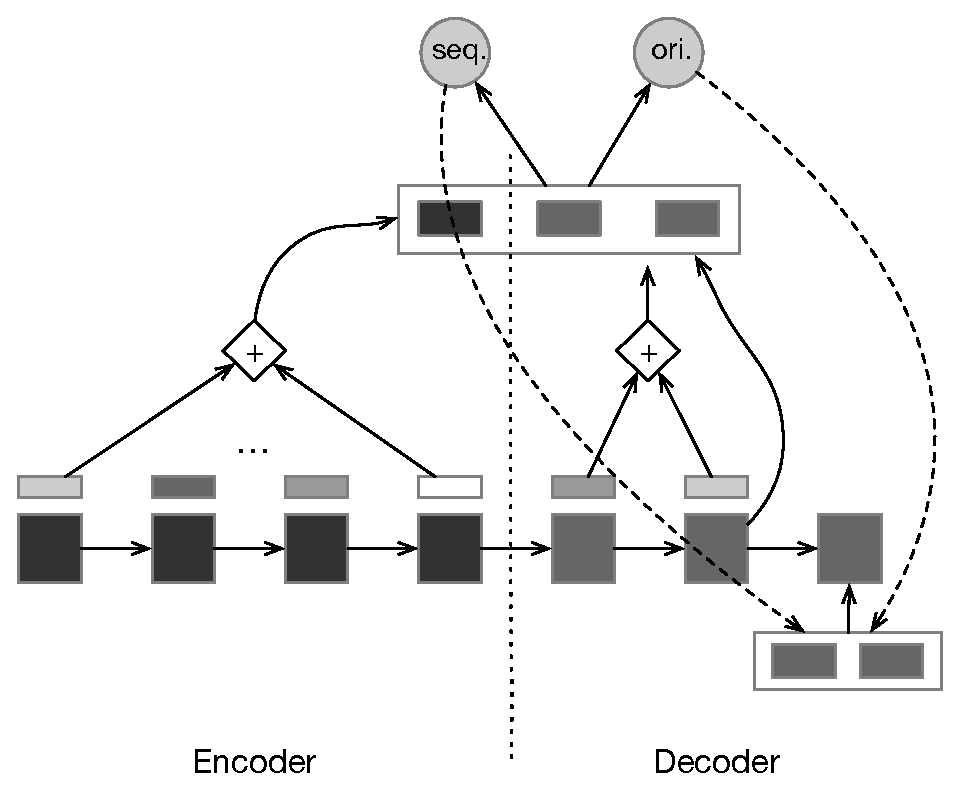
\epsfig{file=binpacking.eps, width=1.0\columnwidth}
	\caption{Architecture for multi-task binpacking networks. }
	\label{fig:architecture-model}
	\vspace{-10pt}
\end{figure}


\subsection{Sequence Task}
\label{sec:sequence_task}
Due to the particularity of the new type 3D BPP problem, it's not allowed to pack the same item repeatedly. The way to prevent the sequence from containing the same item 
twice in the previous work \cite{Hu2017Solving} is a hard constraint and 
it seems that the information of the generated subsequence has no effect on 
the next probability distribution of items.
%Even though this method has generated a better sequence to pack the items, it's unreasonable \yu{confused}.
Obviously, incorporating the information of previous decoding steps into the decoder can help us to generate more reasonable and structured pointers.   
Moreover, taking previously decoded items into consideration means that the network has a priori knowledge to try to avoid repetition to some extend.
To achieve this, we introduce an intra-attention mechanism \cite{paulus2017deep}, which is first proposed to solve the current combinational optimization problem. 

For notation purposes, let us define encoder and decoder hidden states as $h_{i}^{e}$ and $h_{t}^{d}$ respectively. 
Here $h_{i}^{e}$ and $h_{t}^{d}$ are computing from the embedding vector of $x_{i}$ and $y_{t}$ respectively.
We define $attn_{tj}^{d}$ as the intra-attention score of the previous hidden output state $h_{j}^{d}$ at decoding step t:
\begin{eqnarray*}\label{1}
	&attn_{tj}^{d} = softmax(v^{T}tanh(W_{1}h_{j}^{d} + W_{2}h_{t}^{d})),\quad j \in \{1,\dots,t-1\}.
\end{eqnarray*}
Thus, the intra-attention feature $f_{intra}^{t}$ of the current decoded item $s_{t}$ is calculated by using the computed intra-attention weights, for $t > 1$: 
\begin{eqnarray*}\label{2}
	&f_{intra}^{t} = \sum_{j=1}^{t-1}{attn_{tj}^{d}h_{j}^{d}},	
\end{eqnarray*}
where $W_{1}$, $W_{2}$ and $v$ are trainable parameters for intra-attention. Especially for the first decoder cell, we set $f_{intra}^{1}$ to a vector of zeros since the already generated sequence is empty.

The previous intra-attention mechanism is either used to modify the underlying LSTM function \cite{cheng2016long} or to be applied to abstract summarization problems \cite{paulus2017deep}.
To our knowledge, this work is the first to propose this method to solve combinatorial optimization problems.

In previous DRL method for the new type 3D BPP, the pointer mechanism uses the encoder attention weights as the probability distribution to copy the input item. However, in our work, we get the final attention weights $p(s_{t})$ by integrating intra-attention feature at decoder step. In addition, $u_j^t$ is intermediate result which will be normalized by softmax to be the ``attention'' mask over the inputs. 
\begin{eqnarray*}\label{3}
	%	\begin{array}{m}
	&u_{j}^{t} = {v^{'}}^{T}tanh(W_{3}h_{j}^{e} + W_{4}h_{t}^{d} + W_{5}f_{intra}^{t}) \nonumber, \\
	&p(s_{t}) = softmax(u^{t}), \quad j\in\{1,2,...,n\},	 %\eqno(3)   
	%	 \end{array}
\end{eqnarray*}
where $W_{3}$, $W_{4}$, $W_{5}$ and $v^{'}$ are trainable parameters for pointer networks.
We refer all parameters for sequence task as $\theta_{seq}$ and the probability distribution output of sequence task as $p_{\theta_{seq}}(\cdot|\bi{x})$ in the following discussions.

\subsection{Orientation Task}
% Why Multi-task Learning and what's multi-task in our problem?
When placing a cuboid-shaped item, there are 6 orientations, for which we have 3 choices in the first dimension and 2 in the second. For new type 3D BPP, these 6 kinds of orientations are defined as: front-up, front-down, side-up, side-down, bottom-up and bottom-down. For orientation generation, the decoder computes the orientation based on a context vector $\bi{c}$,
which describes the whole problem and is based on the partial solution constructed so far. That is the context of the decoder at time step $t$ comes from the encoder outputs and the output up to time step $t$. For each time step $t$, we calculate the context vector:
\begin{eqnarray*}\label{4}
 	c_t = [h^{e};h_{t}^{d};f_{intra}^{t}].
\end{eqnarray*}
Here, [.;.;] denotes vector concatenation,
$h^{e}$ donates the representation of input sequence and is calculate by an attention-polling function which is defined as follows:
\begin{eqnarray*}
	&h^{e} = \sum_{j=1}^{n}{att_{tj}^{d} * h_{j}^e}, \\
	&attn_{tj}^{d} = softmax({v^{''}}^{T}tanh(W_{6}h_{j}^{e} + W_{7}{[h_{t}^{d};f_{intra}^{t}]})), \\
	& j \in \{1,\dots,n\}.
\end{eqnarray*}
Where $W_{6}$, $W_{7}$ and $v^{''}$ are trainable parameters for attention-polling function.

Thus, the probability distribution of orientations for the current decoding step $t$ is generated by as follows:
\begin{eqnarray*}\label{5}
	p(o_{t}) = softmax(W_{ori}c_t + b_{ori}),
\end{eqnarray*}
where $W_{ori}$ and $b_{ori}$ are trainable parameters for orientations output task.

We define $\bi{o}^{*} = \{o_{1}^{*},o_{2}^{*}, ..., o_{n}^{*}\}$ as the ground-truth orientation sequence for a given input $\bi{x}$ and generated packing sequence $\bi{s}$. As a matter of fact, $\bi{o}^{*}$ is calculated by the Algorithm \ref{Least surface Area Heuristic} in Appendix \ref{NBPH} %\kz{which appendix?}) 
using the placement sequence generated by our sequence task model mentioned above.
%\yu{rephrase the following.}
At each step, least surface area heuristic exhaustively search all possibilities of given free space set and orientation to find the one with least surface area for the current item.  

As we apply supervised training in this part, the objective is to maximize the likelihood of all orientation labels $\bi{o}^{*}$ , given the generated placement sequence $\bi{s}^{'}$ and model parameters $\theta_{ori}$ for orientation task:
\begin{eqnarray*}
	\log{p(\bi{o}^{*}|\bi{s}^{'}, \theta_{ori})} = \sum_{i=1}^{n}\log{p(o_{i}^{*}|s_1,\dots,s_{i-1}, \theta_{ori}, \bi{x})}.
\end{eqnarray*}

Besides, We refer the probability distribution output of orientation task as $p_{\theta_{ori}}(\cdot|\bi{x})$ in the following discussions.

\subsection{Training and Testing}
\label{sec:training_Testing}
In this subsection, we will illustrate the training and testing procedure which is specially designed for our new type 3D BPP.
\subsubsection{Training}
\label{sec:train}

To train a multi-task model, we use a hybrid loss function to combine supervised learning and reinforcement learning.
For sequence task, we use REINFORCE algorithm \cite{williams1992simple} as before in \cite{Hu2017Solving}. However, for orientation task, the orientation is chosen stochastically from a distribution parameterized by supervised learning. Nevertheless, as the orientation task is much more complex than the sequence, the sequence task will suffer from the bad initializer of orientation if they are trained at the same time. To overcome this shortcoming, pre-training the orientation task first could be a reasonable idea.
However, orientations of the items is tightly attached to the existence of packing sequence of items in new type 3D BPP. 
Consequently, we train different types of tasks separately for each random batch to keep them dynamic balance.
We called this \textbf{M}ulti-\textbf{t}ask \textbf{S}elected \textbf{L}earning (MTSL). Mathematically, there are three kinds of basic loss function in our work:
\begin{eqnarray*}
	%\begin{array}{m}
	&p(s_{i}) = {p(s_{i}|s_{1},o_{1}^{*}, ..., s_{i-1}, o_{i-1}^{*}, \theta_{seq}, \bi{x})},\\
	&L_{seq} = (SA(\bi{s},\bi{o}|\bi{x}) - bl(\bi{x}))\sum\limits_{i=1}^{n}\log{p(s_{i})},\\
	& L_{ori} = -\sum\limits_{i=1}^{n}\log{p(o_{i}^{*}|s_{1}, o_{1}^{*}, ..., s_{i-1}, o_{i-1}^{*}, s_{i}, \theta_{ori}, \bi{x})},\\
	&L_{all} = L_{seq} + L_{ori},
	%\end{array}
\end{eqnarray*}
where $SA(\bi{s},\bi{o})$ denotes the surface area of the bin in the case of 
placement sequence and its corresponding orientation of $\bi{o}$ and $\bi{s}$, 
and $bl(\bi{x})$ denotes the baseline surface area by a well-designed algorithm NBPH.  %\yu{definition}.  %(see appendix \kz{What?}). 
During training, our model will choose one of the three kinds of loss $\{L_{seq}, L_{ori}, L_{all}\}$
to balance difficulty among them with a certain probability.  

\subsubsection{Baseline iteration: Exponential Moving Average}
For sequence task, as we use the REINFORCE estimator with baseline, a good baseline reduces the variance of the estimator and increases the convergence speed of learning. In our work, we resort a baseline iteration as there is no need to differentiate between inputs and simple to implement, rather than critic. For an sample $\bi{x}$, the baseline value $bl(\bi{x})$ is initialized by calculating the surface area of a packing plan which is generated by the heuristic algorithm NBPH. In each step, the baseline value is updated as:
\begin{eqnarray*}
	bl'(\bi{x}) = SA(\bi{s},\bi{o}|\bi{x}) + \alpha(bl(\bi{x})-SA(\bi{s},\bi{o}|\bi{x})),
\end{eqnarray*}
where $SA(\bi{s},\bi{o}|\bi{x})$ is the surface area calculated at each training step and $\alpha$ is the hyper-parameter for exponential moving average.

As a conclusion of the discussion above, the training procedure of our Multi-task Selected Learning method can be summarized in Algorithm \ref{alg-summary-drl}.

\begin{algorithm}                  % enter the algorithm environment
	\caption{Multi-task Selected Learning.}       
	\label{alg-summary-drl} 
	\begin{algorithmic}[1]
		\State Training set $X$, number of training steps $T$, batch size $B$.
		\State Initialize Sequence and Orientation parameters $\theta_{seq}$, $\theta_{ori}$.
		\State Initialize baseline value $bl$ according to NBPH.
		\For {\emph{t = 1 to T}}
		\State Select a batch of samples $\bi{x}$ and calculate baseline $bl(\bi{x})$.
		\State Sample solution $\bi{s}$ by sequence task probability $p_{\theta_{seq}}(\cdot|\bi{x})$ .
		\State Obtain free space $\bi{f}$ and orientation $\bi{o}^{*}$ for $\bi{s}$ by Algorithm \ref{Least surface Area Heuristic}
		\State Calculate $SA(\bi{s},\bi{o}^{*}|\bi{x})$ by tuple $(\bi{s},\bi{o}^{*},\bi{f})$
		\State %$g_{\theta_{seq}}=\frac{1}{B}\sum\limits_{k=1}^{B}\nabla_{\theta_{seq}}\log{p(s_{t,k}|s_{t,1},o_{t,1}^{*},\dots,s_{t,k-1},o_{t,k-1}^{*},x_t)}*(SA(s_t, o_{t}^{*}|x_t)-bl(x_t)) $
		$g_{\theta_{seq}}=\mathbb{E}[(SA(\bi{s}, \bi{o}^{*}|\bi{x})-bl(\bi{x}))\nabla_{\theta_{seq}}\log{p(\bi{s}|\bi{x})}]$
		\State  %$g_{\theta_{ori}}=\frac{1}{B}\sum\limits_{k=1}^{B}\nabla_{\theta_{ori}}\log{p(o_{k}^{*}|s_{t,1},o_{t,1}^{*},\dots,s_{t,k-1},o_{t,k-1}^{*},x_t)}$
		$g_{\theta_{ori}}=\mathbb{E}[\nabla_{\theta_{ori}}\log{p(\bi{o}^{*}|\bi{x})}]$
		\State 	$g_{\theta_{all}}= g_{\theta_{seq}}+g_{\theta_{ori}}$.
		\State  $g_{\theta} = choice(g_{\theta_{seq}},g_{\theta_{ori}},g_{\theta_{all}})$
		\State Update $\theta = ADAM(\theta, g_{\theta})$.
		\State Update baseline $bl(\bi{x}) = SA(\bi{s},\bi{o}^{*}|\bi{x}) + \alpha(bl(\bi{x})-SA(\bi{s},\bi{o}^{*}|\bi{x}))$.
		\EndFor
		\State return all parameters $\theta_{seq}$, $\theta_{ori}$.
	\end{algorithmic}
\end{algorithm}


\subsubsection{Testing}
\label{sec:test}
Moreover, different from traditional machine learning problems, combinational optimization problem are to minimize or maximize the objective under some constraints, which seems to have some of priori knowledge about how to evaluate the result.
 For our new type 3D BPP, the benchmark is the smaller the better. As evaluating a surface area is inexpensive, we can simply generate multiple candidate solutions per order at inference time and select the best. The way generates  candidates is based on the calculated probability $p_{\theta_{seq}}(\cdot|\bi{x})$ and $p_{\theta_{ori}}(\cdot|\bi{x})$. Meanwhile, as we can only obtain the packing sequence and orientation for each order , we still need Algorithm \ref{Least surface Area Heuristic(1)} in Appendix \ref{NBPH} to get the free space set for calculating the surface area.%Besides, the same procedure training and testing This harmonizes learning with the inference procedure, and lowers the variance of the gradients, improving the training procedure.  

